\begin{figure*}
	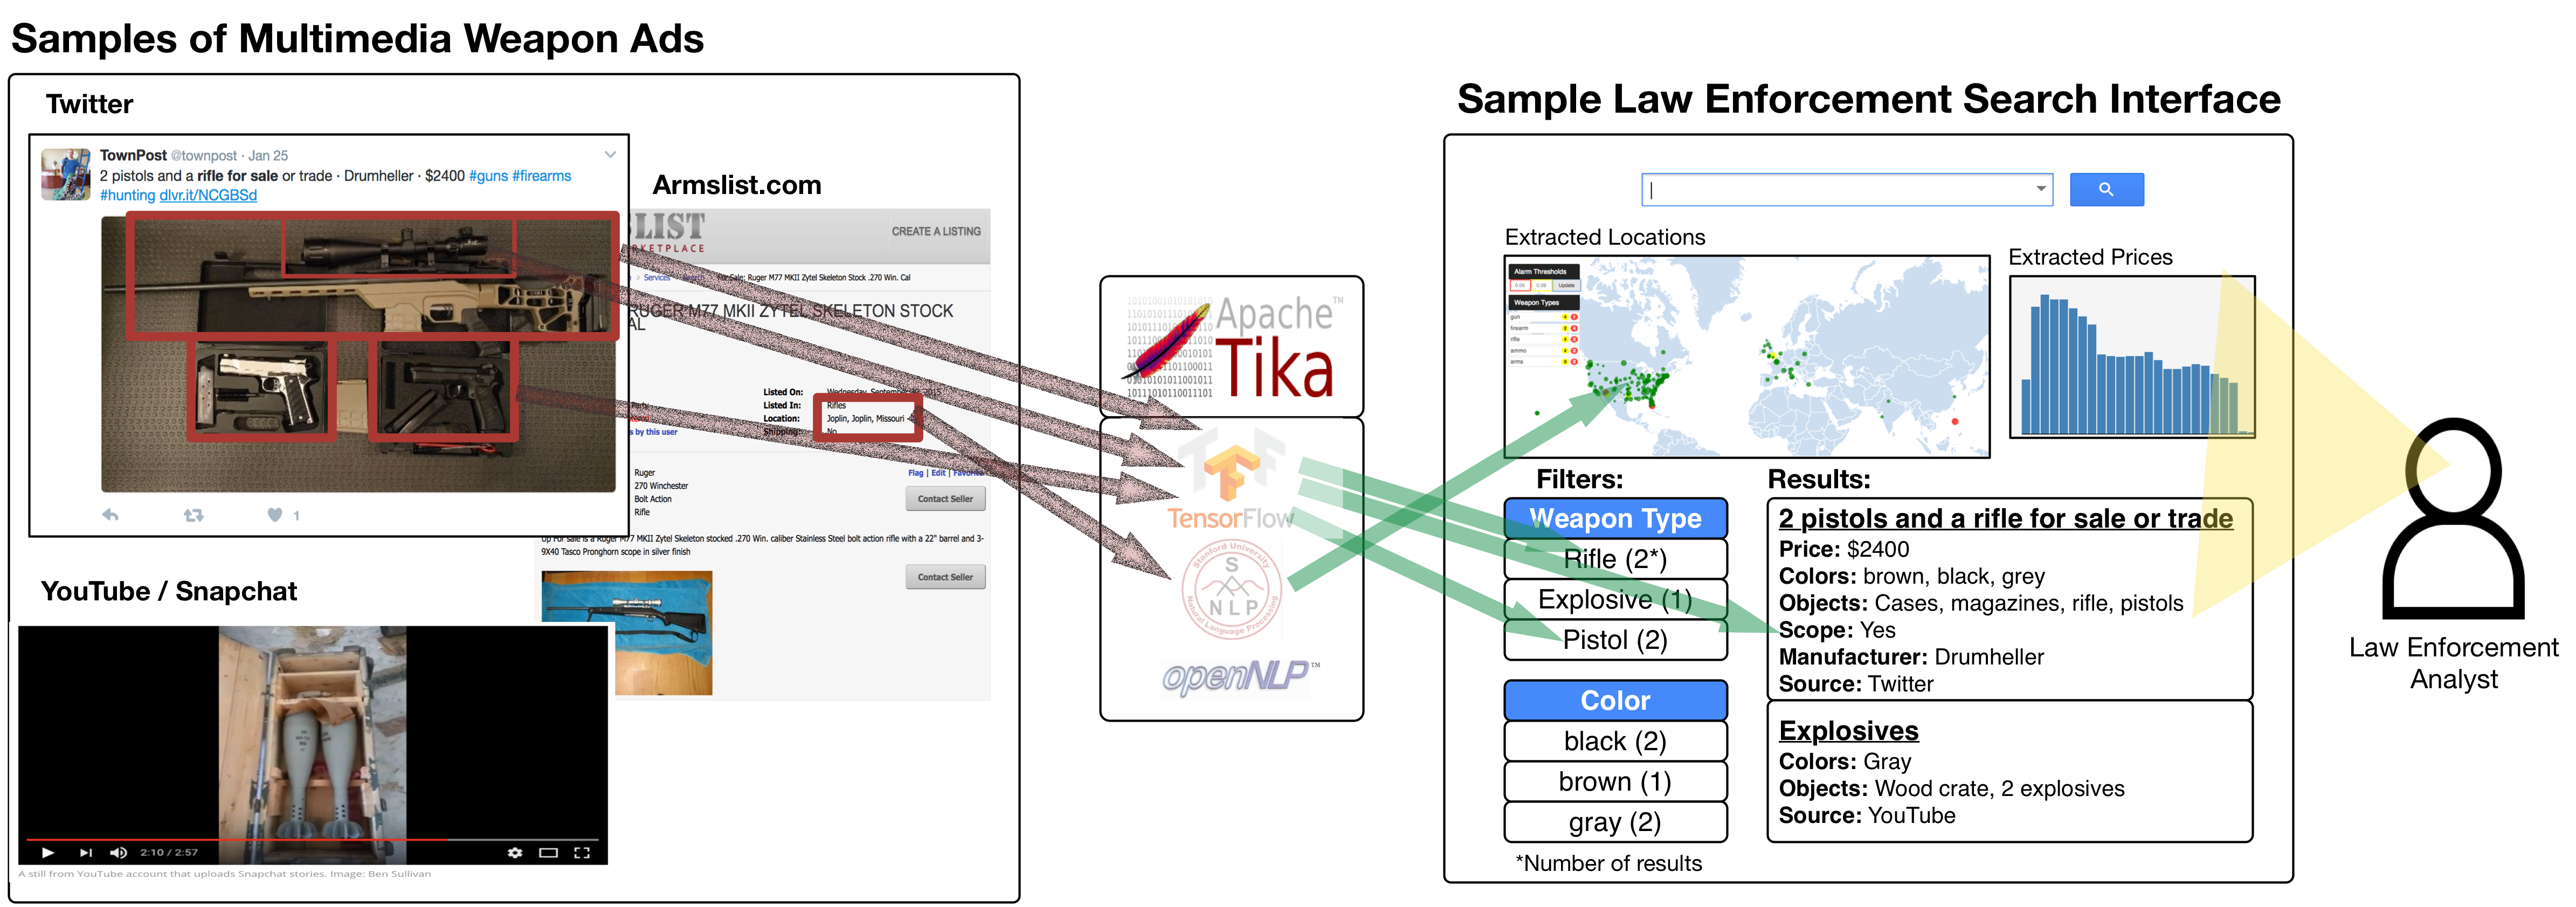
\includegraphics[width=\textwidth,height=6cm]{interface-diagram}
	\caption{This diagram demonstrates how the integration of Tika and Tensorflow facilitates interfaces in-depth search across heterogenuous content types. There are several extensions to our object recognition implementation as well, including more refined categories, optical-character recognition, and image similarity metrics.}
	\label{fig:interface-diagram}
\end{figure*}

\section{CONTENT ANALYSIS IN MEMEX PROGRAM} \label{sec:memex}
This section discusses the background and motivations of DARPA Memex program and its datasets. The current commercial web search engines provides a generalized search interface to all users~\cite{}. However, in the context of cyber security, the commercial search engines miss resources from the deep and dark web which are essential for law keeping agencies. The goal of Memex program is to develop softwares that can quickly and thoroughly organize and search subsets of information relevant to the individual interests. The first two interests were in the domains of human trafficking and illegal weapon sale.

\subsection{Data Collection}
\label{sec:memex-datacollection}
Several web crawlers were used to discover and retrieve information from the websites.
Along with the general-purpose web crawlers, there was specialized crawler for the retrieval of dark data using TOR protocol \cite{} and also specialized in the retrieval of dynamic AJAX content guarded by login forms. The fetched data were cached within the system for analysis due to the ephemeral nature of the content at the sources.

\subsection{Memex Dataset} \label{sec:memex-dataset}
The dataset used in our experiment was a subset of memex dataset in public domain. It contained 7.2 million documents in the illegal weapon sales domain in which 1.4 million documents were images. We had analyzed the textual documents and the named entities separately in a different experiment using named entity recognition models and extractors for people, location, organization, weapon name, and weapon-types. In this experiment, we were interested in labeling images by classifying them into various classes. Usually, web crawlers fetch all resources linked in the web pages and hence classification was an important pre-processing to remove noise for the later analysis.

\subsection{Tools for Law Enforcement} \label{sec:memex-tools}
The ultimate goal of integrating diverse content scattered across the web is to provide law enforcement analysts with tools that will help them quickly identify relevant information. In the context of Memex, multimedia content is essential in helping analysts sift through millions of ads in search of illicit sales; images and videos often provide salient information not available in text. In many cases, illegal weapons dealers intentionally embed revealing details in rich content mediums because they are harder to identify. This thinking coincides with the rise of weapons trafficking on social media platforms such as Snapchat, YouTube, and Instagram, where communication is centered around images and video \cite{socialmedia}. The integration of Tensorflow and Tika provides a single, streamlined platform that unites the extraction of textual and rich content. This combined content can then be exposed through search and visualization interfaces that improve analysts' abilities to drill-down and explore comprehensive, diverse content contained in weapons ads (see Figure). Our use of Tensorflow and the Inception-V3 model serves as an example of the benefits of this integration and the types of insights and capabilities it facilitates in the future. 